\documentclass[11pt,letterpaper,boxed]{hmcpset}
\usepackage{fullpage}
\setlength{\parskip}{6pt}
\setlength{\parindent}{0pt}
\usepackage[margin=1in]{geometry}
\usepackage{graphicx}
\usepackage{enumerate}
\usepackage{marvosym}
\usepackage{amssymb}
\usepackage{wasysym}
\usepackage{gensymb}
\usepackage{mathrsfs}
\usepackage{scrextend}
\usepackage{mathtools}
\usepackage{pgfplots}
\usepackage{xspace}
\usepackage{esvect}
\usepackage{lipsum}
\usepackage{float}


\name{Name $\rule{4cm}{0.15mm}$}
\class{Physics 51M Section $\rule{.5cm}{0.15mm}$ Box \# $\rule{1cm}{0.15mm}$}
\assignment{Problem Set 3}
\duedate{23 September 2019}

\begin{document}
	
	%\begin{center}
	\noindent\textbf{Collaborators:} 
	%\end{center} 
	
	%\problemlist{}
	
	\begin{problem}[Schey II-8] 
		An electrostatic force field is given by $\vec{E} = \lambda (\vec{\textbf{i}}yz + \vec{\textbf{j}}xz + \vec{\textbf{k}}xy)$, where $\lambda$ is a constant. Use Gauss' law to find the total charge enclosed by the surface shown in the figure consisting of $S_1$, the hemisphere $z = (R^2 - x^2 - y^2)^{\frac{1}{2}}$, and $S_2$, its circular base in the $xy$-plane.
		\begin{center}
			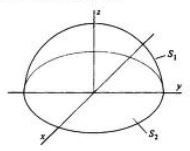
\includegraphics[scale=0.9]{51m3pic2.jpg}
		\end{center}
		
	\end{problem}
	
	\begin{solution}
		\vfill
	\end{solution}
	\newpage

	\begin{problem}[Schey II-10] 
		It sometimes happens that surface integrals can be evaluated without using the long-winded procedures outlined in the text. Try evaluating $\iint_S \vec{\textbf{F}} \cdot \hat{\textbf{n}}\,dA$ for each of the following; think a bit and avoid a lot of work!
		
		\begin{enumerate}
			\item [(a)] $\vec{\textbf{F}} = \vec{\textbf{i}}x + \vec{\textbf{j}}y + \vec{\textbf{k}}z$. 
				\\$A$, the three squares each of side $b$ as shown in the figure.
			\item [(b)] $\vec{\textbf{F}} = (\vec{\textbf{i}}x + \vec{\textbf{j}}y)\ln(x^2+y^2)$. 
				\\$A$, the cylinder (including the top and bottom) of radius $R$ and height $h$ shown in the figure.
			\item [(c)] $\vec{\textbf{F}} = (\vec{\textbf{i}}x + \vec{\textbf{j}}y + \vec{\textbf{k}}z)e^{-(x^2+y^2+z^2)}$. 
				\\$A$, the surface of the sphere of radius $R$ centered at the origin as shown in the figure.
			\item[(d)] $\vec{\textbf{F}} = \vec{\textbf{i}}E(x)$, where $E(x)$ is an arbitrary scalar function of $x$.
				\\$A$, the surface of the cube of side $b$ shown in the figure.
		\end{enumerate}
		\begin{center}
			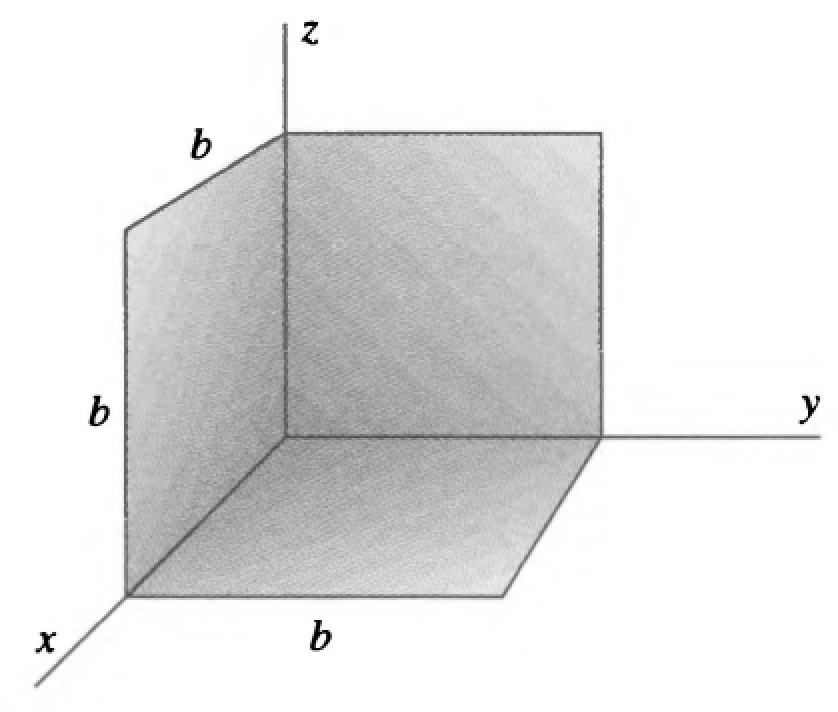
\includegraphics[scale=0.25]{II-10a.png}
			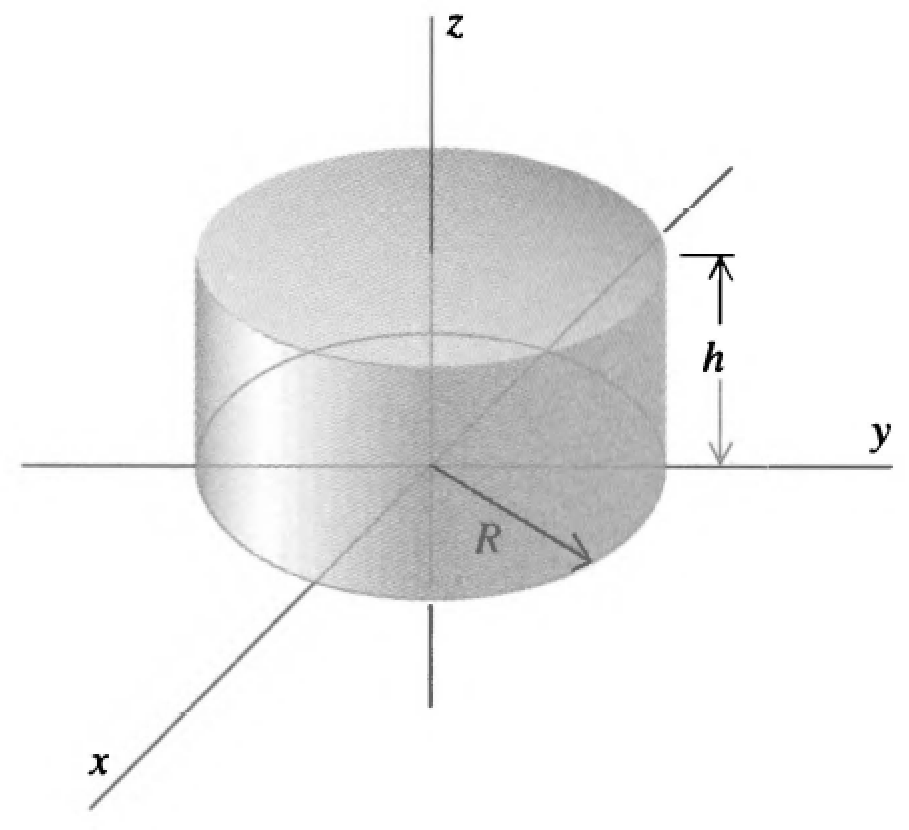
\includegraphics[scale=0.25]{II-10b.png}
			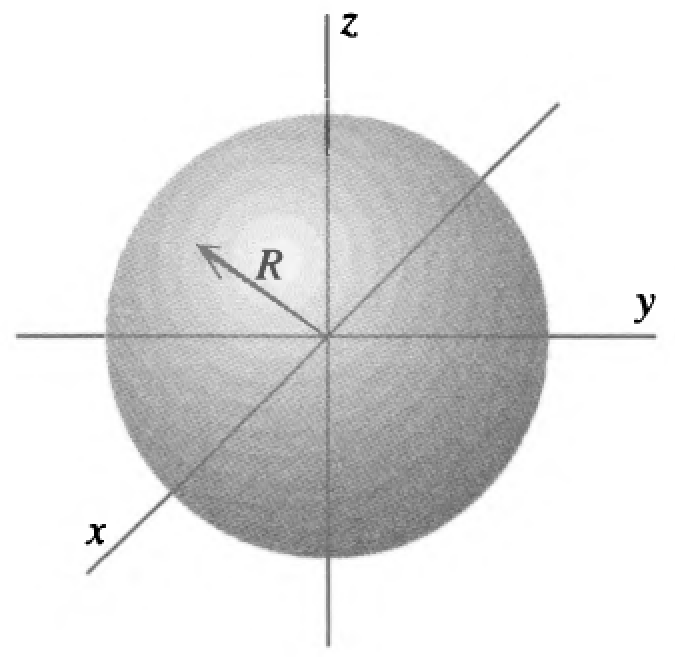
\includegraphics[scale=0.25]{II-10c.png}
			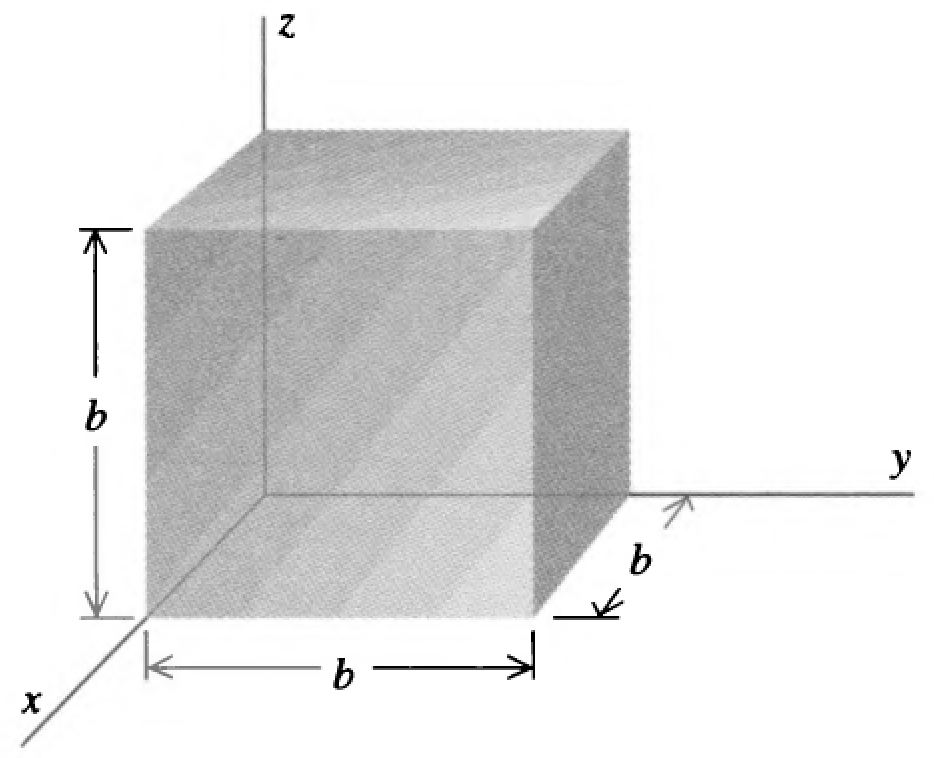
\includegraphics[scale=0.25]{II-10d.png}
			\\Figures (a), (b), (c), and (d)
		\end{center}
			
		
	\end{problem}
	
	\begin{solution}
		\vfill
	\end{solution}
	\newpage

	\begin{problem}[HRK E27.11]
		A point charge $q$ is placed at one corner of a cube of edge $a$. What is the flux through each of the cube faces? (Hint: Use Gauss' law and symmetry arguments.)
		
	\end{problem}
	
	\begin{solution}
		\vfill
	\end{solution}
	\newpage	
	
	\begin{problem}[HRK E26.40]
		Figure 26-36 shows a Thomson atom model of helium $(Z = 2)$. Two electrons, at rest, are embedded inside a uniform sphere of positive charge $2e$. Find the distance $d$ between the electrons so that the configuration is in static equilibrium.
		
		\begin{center}
			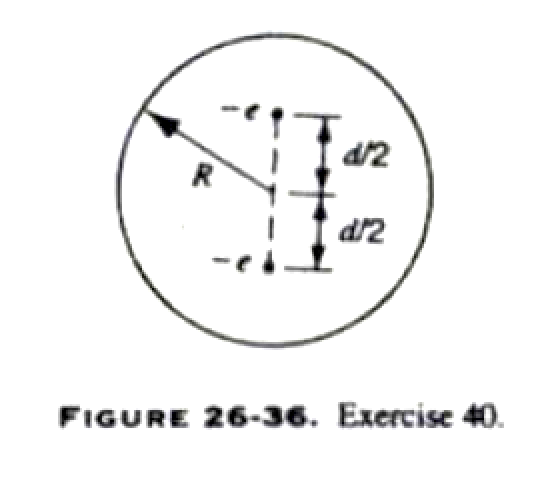
\includegraphics[scale=0.55]{26-36.png}
		\end{center}
		
	\end{problem}
	
	\begin{solution}
		\vfill
	\end{solution}
	\newpage
	
	\begin{problem}[HRK P27.17]
		A solid nonconducting sphere of radius $R$ carries a nonuniform charge distribution, with charge density $\rho$ = $\rho_s r/R$, where $\rho_s$ is a constant and $r$ is the distance from the center of the sphere. Show that
		\begin{enumerate}
			\item[(a)]the total charge on the sphere is $Q = \pi\rho_s R^3$
			\item[(b)]the electric field inside the sphere is given by $E = \frac{1}{4\pi\epsilon_0}\frac{Q}{R^4}  r^2$
			\item[(c)]Write down the electric field outside the sphere, $r > R$. You do not need to derive your result, just explain how you know what it is.
		\end{enumerate}
		
		
	\end{problem}
	
	\begin{solution}
		\vfill
	\end{solution}
	\newpage
	
	\begin{problem}[HRK E27.25]
	\\Charge is distributed uniformly throughout an infinitely long cylinder of radius $R$. 
		\begin{enumerate}
			\item[(a)] Show that $E$ at a distance $r$ from the cylinder axis ($r < R$) is given by $E = \frac{\rho r}{2\epsilon_0}$, where $\rho$ is the volume charge density.
			\item[(b)] What result do you obtain for $r > R$?
		\end{enumerate}
		
	\end{problem}
	
	\begin{solution}
		\vfill
	\end{solution}
	\newpage
	
	
\end{document}